% This syllabus template was created by:
% Brian R. Hall
% Assistant Professor, Champlain College
% www.brianrhall.net

% Document settings
\documentclass[11pt]{article}
\usepackage[margin=1in]{geometry}
\usepackage[pdftex]{graphicx}
\usepackage{multirow}
\usepackage{setspace}
\usepackage{listings}
\pagestyle{plain}
\setlength\parindent{0pt}

\begin{document}
	
	\subsection*{Machine thermique} 
	Une machine thermique transforme la chaleur (issue le plus souvent de la combustion du charbon, du bois, du gaz, de l’essence, etc.) en travail mécanique.
	
	Exemple : la machine à vapeur. L’eau est chauffée jusqu’à ébullition, la vapeur se détend et pousse un piston. Ensuite, la vapeur se condense et l’eau est rejetée. Le cycle recommence avec une nouvelle quantité d’eau prélevée dans le réservoir.
	
	Important : la machine doit être cyclique, c’est-à-dire revenir à son état initial à chaque cycle.
	
	\subsubsection*{Modèle simplifié d'une machine thermique}
	On ne rentre pas dans les détails de la combustion. Il y a une source chaude, une source froide, et la machine fonctionne entre ces deux sources.
	
	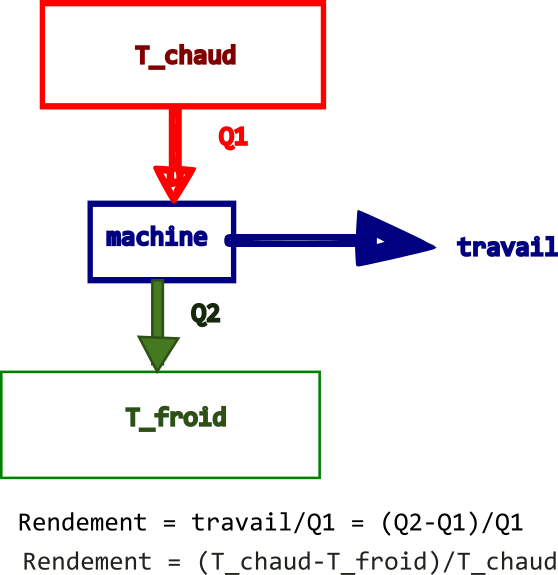
\includegraphics[width=0.7\linewidth]{images/machine_thermique.png}
	
	Ce qui est important, c’est la limitation du rendement d’une machine thermique, même idéale (sans pertes dues aux frottements).
	
	La machine thermique peut être inversée : c’est le principe du réfrigérateur et de la pompe à chaleur.
	
	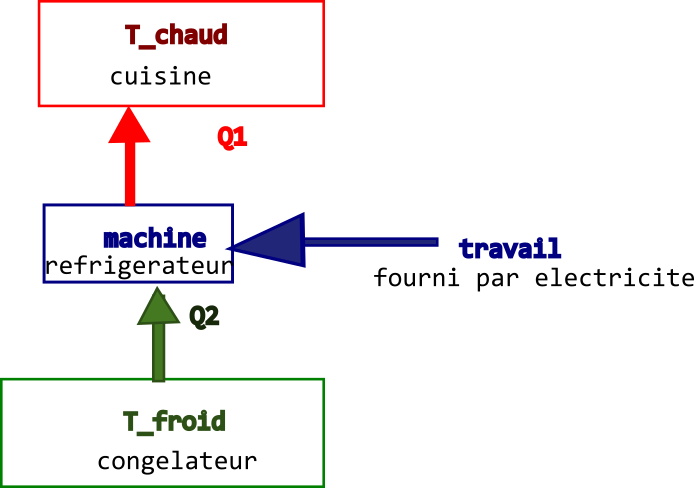
\includegraphics[width=0.7\linewidth]{images/machine_thermique_inv.png}
	
	\subsection*{Notion d'entropie}
	
	L’entropie est une grandeur thermodynamique qui mesure le degré de désordre ou de dispersion de l’énergie dans un système.
	
	Elle est notée $S$ et s’exprime en joules par kelvin (J/K).
	
	\begin{itemize}
		\item Faible entropie : système ordonné (solide, liquide)
		\item Forte entropie : système désordonné (gaz)
	\end{itemize}
	
	Pour une transformation réversible :
	\begin{equation}
		\Delta S = \frac{Q}{T} 
	\end{equation}
	
	où $Q$ est la chaleur échangée avec le système.
	Pour une transformation irréversible :
	\begin{equation}
		\Delta S > \frac{Q}{T} 
	\end{equation}
	Si le système est thermiquement isolé et que la transformation est réversible (donc lente), elle est dite adiabatique. Une telle transformation est aussi isentropique.
	
	Si la transformation est irréversible (par exemple, échange de chaleur avec une grande différence de température ou présence de frottements), l’entropie du système augmente.
	\subsubsection*{L’entropie est une fonction d’état du système}
	
	Cela signifie que, quelle que soit la manière dont le système a atteint son état actuel, l’entropie est la même.
	
	En revanche, la chaleur échangée n’est pas une fonction d’état : on peut atteindre un même état final par des chemins différents, impliquant des échanges de chaleur et/ou du travail différents.
	\subsection*{Deuxième principe de la thermodynamique}  
	Il existe deux formulations équivalentes.
	
	\subsubsection*{Formulation 1}
	L’entropie d’un système isolé ne peut pas diminuer.
	
	\subsubsection*{Formulation 2}
	Un processus dont le seul résultat serait le transfert de chaleur d’un corps froid vers un corps chaud est impossible.
	
	\subsection*{Transformation isentropique d'un gaz parfait}
	Une transformation isentropique est une transformation au cours de laquelle l'entropie reste constante :
	\[
	s =  const 
	\]
	
	Pour un gaz parfait, cela correspond à une transformation adiabatique réversible.  
	Les paramètres du gaz obéissent à la relation :
	
	\[
	p V^{\gamma} =   const 
	\]
	
	c’est-à-dire, pour une transformation de $(P_1, V_1)$ à $(P_2, V_2)$ :
	\[
	P_1 V_1^{\gamma} = P_2 V_2^{\gamma}
	\]
	
	où $\gamma$ est appelé l’indice adiabatique. Il peut être déterminé théoriquement par la physique statistique, qui étudie le comportement des molécules.  
	Pour un gaz parfait monoatomique : $\gamma = 5/3$,  
	pour un gaz parfait diatomique : $\gamma = 7/5$.
	
	\subsection*{Remarques}
	
	\begin{itemize}
		\item Transformation adiabatique : \( Q = 0 \)
		\item Transformation réversible : pas de création d'entropie
		\item Compression : la température augmente
		\item Détente : la température diminue
	\end{itemize}
 
	
\end{document}
 
 



